\chapter{Hardware Accelerator}

The Raspberry Pi 5 with an Ai kit was chosen as the hardware to prove the concept of computing data at the edge.
This desiction was taken based on recommendations from the advisors and the avilability.
The market analysis confirms this choice.
The hardware accelerator of the Ai kit is made by Hailo \cite{hailo}.
Hailo is a company which produces hardware accelerators.
The Ai kit uses the Hailo-8L entry level hardware accelerator.
Hailo provides a pipeline to compile a network so that it can be executed on the hailo software.
First we take a look at the compilation of a network which has to be done on a pc.
Secondly were looking on the way to run the network on the edge.

\section{Network compilation}
As sad before, the network has to be precompiled on a pc.
The application which is meant for this task is callde the \Acrfull{dfc}.

\subsection{Dataflow compiler}

To use the \acrshort{dfc} a pytorch or tensorflow model has to be converted to Onnx or tensorflow light.
Information and pictures are taken from \cite{hailo_dataflow_compiler}.
The \acrshort{dfc} the compiles the model to a \Acrfull{hef} by executing the following steps:
\begin{enumerate}
    \item Tensorflow or ONNX translation
    \item Profiler
    \item Emulator
    \item Model Optimization
    \item Compiling the model into a binary image
\end{enumerate}



\begin{figure}
    \centering
    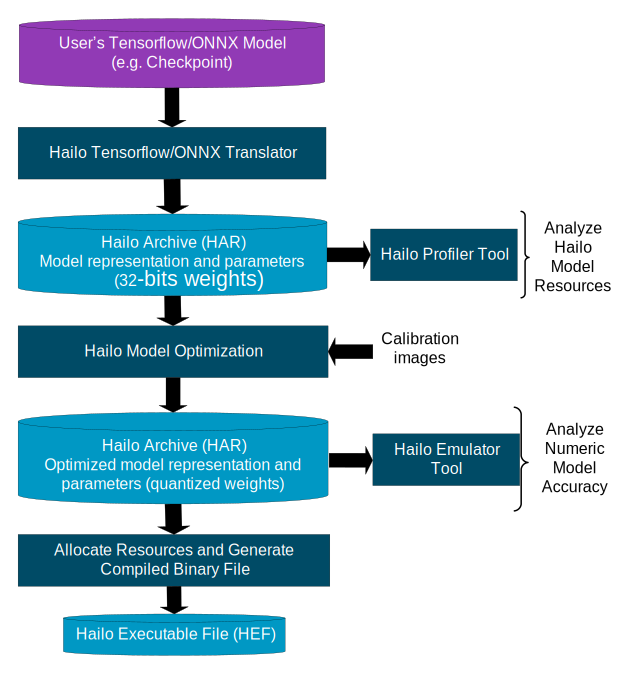
\includegraphics[width=\textwidth]{Images/Hardware/model_build_overview_with_onnx_and_hef_w_har.png}
    \caption{\Acrlong{dfc} overview \cite{hailo_dataflow_compiler}}
    \label{fig:hardware:dfcoverview}
\end{figure}

\subsection{Constrains}
At the time of this writing, the \acrshort{dfc} is not capable of compiling Transformers.
Fortunately, the visual encoding of CLIP can also be done with ResNet, a special form of \Acrshort{cnn}'s.

\section{Running on the edge}

Hailo provides a library called TAPPAS which is based on GStreamer.
The library enables using a Hailo device within gstreamer pipelines t create intelligent video processing applications.
The information for this section are taken from the TAPPAS User Guide.
In the point of time there are 2 approaches to run a network on a hailo device.
One with Gstreamer and one with a Python API.
There are many different example applications available for many diffrent usecases.
Sadly most of the exmaples work with a video input.


\subsection{GStreamer approach}

Gstreamer is a framework for creating streaming media applications.
It enables the design any type of multimedia application but it isnt restridted to audio and video processing.
The framework can porcess any kind of dataflow.

GStreamer consists of blocks which can be concantenated.
To work with the Hailo hardware accelerator some blocks in the pipeline get offloaded to the Hailo porcessor.
A python programm is used to construct a string which then is executed in a terminal.


\subsection{Python API approach}

With the Python API approch one can execute the whole inferance in python.
A thread for the inferance gets created which communicates over queues with the rest of the programm.
That makes the programm very simple in comparison to the GStreamer approach.